%!TEX root = ../main.tex
%%%%%%%%%%%%%%%%%%%%%%%%%%%%%%%%%%% Links: https://www.yumpu.com/en/document/read/7789379/lowest-common-ancestorlca-chair-for-efficient-algorithms
%
% Difficulty:
% Companies: 
%%%%%%%%%%%%%%%%%%%%%%%%%%%%%%%%%%

\chapter{Distance between nodes in BST}
\label{ch:distance_between_nodes_in_tree}
\section*{Introduction}

In the problem described in this chapter  we are going to investigate how we can find the the distance between two nodes in a binary search tree. 
As we will see this problem can be approached and solved very straightforwardly 
if we are able identify the key idea behind it. This insight can become apparent after we look at a few examples and our advice for approaching this problem (and to be honest all problems on graphs and trees)
is to draw and discuss quite a few examples with your interviewer. This help you get a much better intuitive understanding of 
what the problem is really about, which will eventually lead to the eureka moment.

This is going to be a relatively short chapter because the solution is built on top of the solution of a problem discussed in another chapter. 
In Section \ref{sec:distance_between_nodes_in_tree:problem} we will have a look at the formal problem statement 
and in Section \ref{distance_between_nodes_in_tree:sec:discussion} we discuss the solution approach and we will look into two possible different implementations: recursive and iterative. 

\section{Problem statement}
\ref{sec:distance_between_nodes_in_tree:problem}
\begin{exercise}
	Write a function that takes as input a binary search tree $T$ and two nodes $p$ and $q$ and returns the distance between $p$ and $q$.
	The distance between two nodes $D(p,q)$ is defined as the number of edges you need to traverse to get from $p$ to $q$.
	
	\begin{example}
		\hfill \\
		Given the tree shown in Figure \ref{fig:distance_between_nodes_in_tree:example1}, 
		$p = 1$ and $q=3$, the function returns $D(1,3)=2$ 
		
		If $p=3$ and $q=2$ the function returna $1$.
	\label{ex:distance_between_nodes_in_tree:example1}
	\end{example}

	\begin{example}
		\hfill \\
		Given the tree shown in Figure \ref{fig:distance_between_nodes_in_tree:example2}, 
		$p = 5$ and $q=2$, the function returns $D(5,2)=6$ 
		\label{ex:distance_between_nodes_in_tree:example2}
	\end{example}
\end{exercise}

\begin{figure}
	\centering
	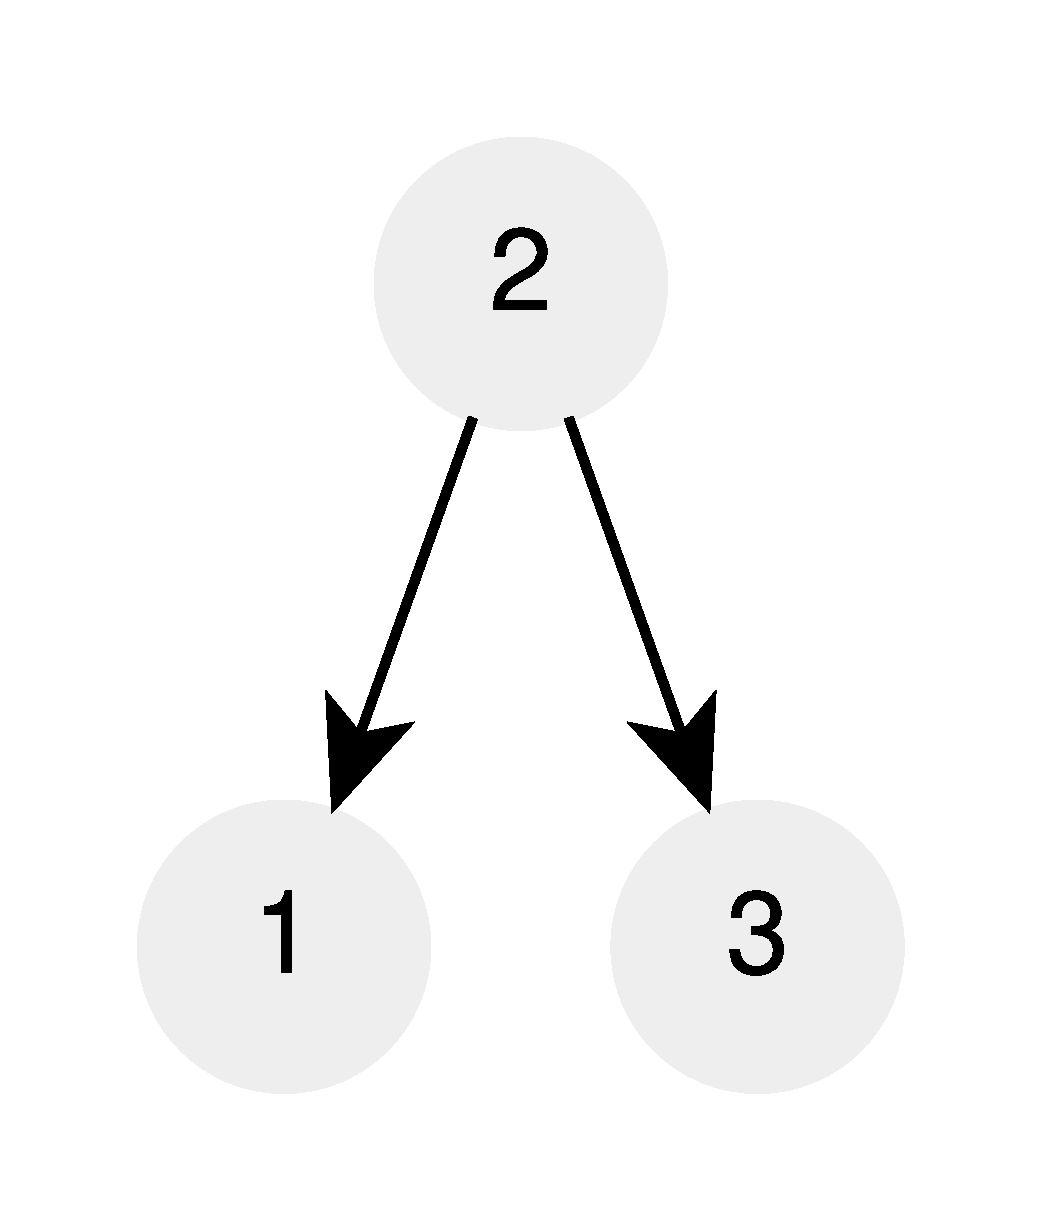
\includegraphics[width=0.3\textwidth]{sources/distance_between_nodes_in_tree/images/example1}
	\caption{Binary Search tree of the Example
	\ref{ex:distance_between_nodes_in_tree:example1}}.
	\label{fig:distance_between_nodes_in_tree:example1}
\end{figure}


\begin{figure}
	\centering
	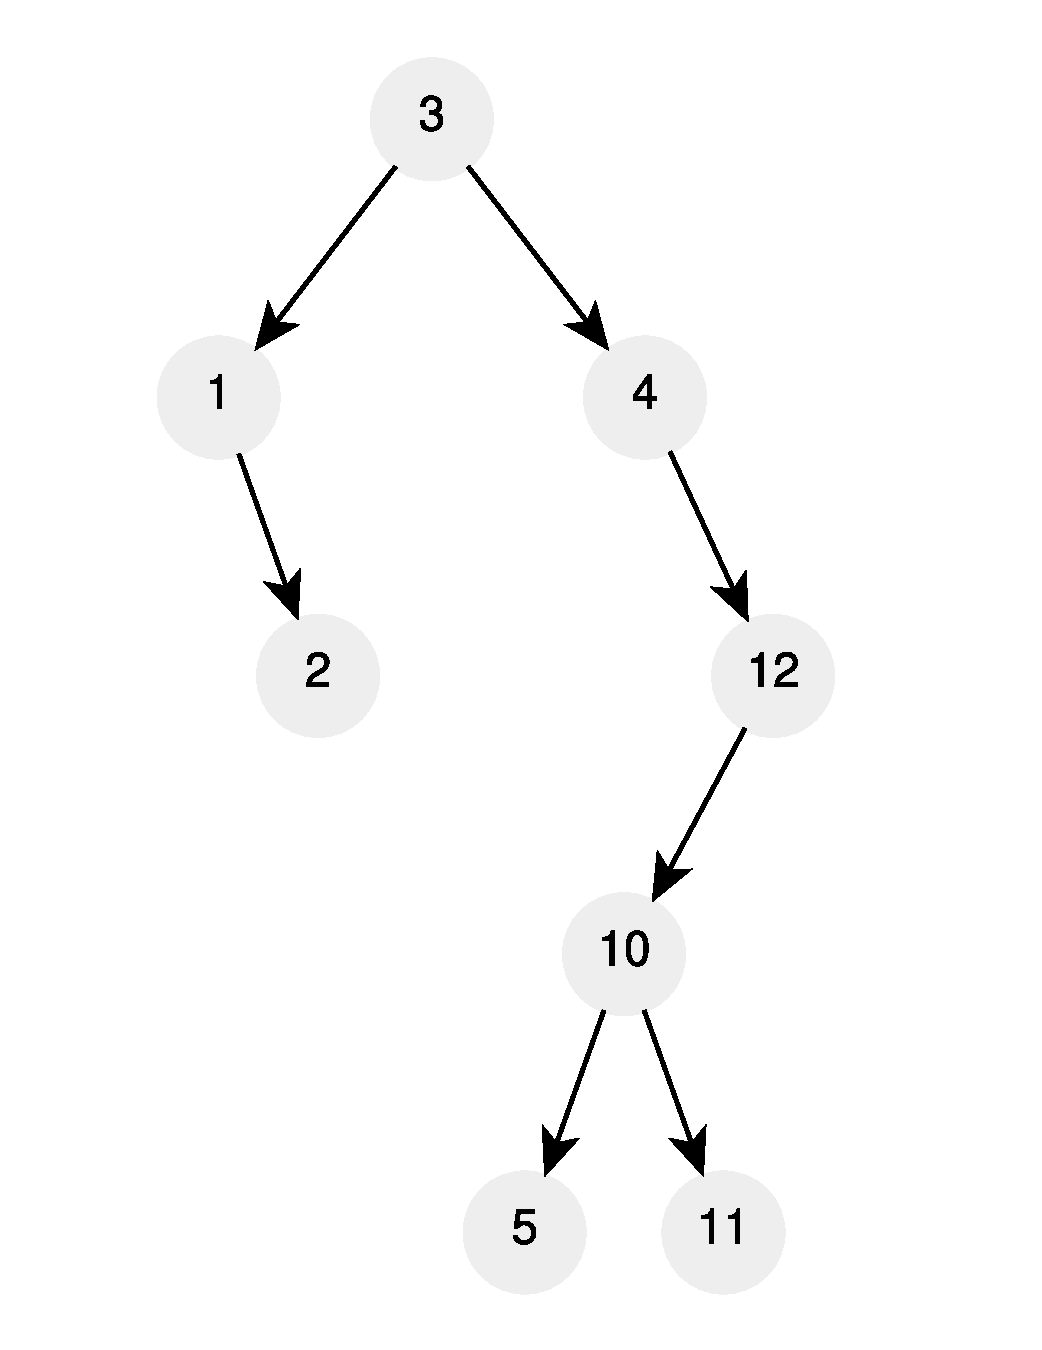
\includegraphics[width=0.5\textwidth]{sources/distance_between_nodes_in_tree/images/example2}
	\caption{Binary Search tree of the Example
	\ref{ex:distance_between_nodes_in_tree:example2}}.
	\label{fig:distance_between_nodes_in_tree:example2}
\end{figure}

\section{Clarification Questions}

\begin{QandA}
	\item Can $p$ be equal to $q$?
	\begin{answered}
		\textit{Yes, this is a valid case.}
	\end{answered}
	
	\item Is it guaranteed for  $p$ and  $q$ to be present in $T$?
	\begin{answered}
		\textit{Yes, you can assume $T$ always contains both $p$ and $q$.}
	\end{answered}

\end{QandA}

\section{Discussion}
\label{distance_between_nodes_in_tree:sec:discussion}
As already mentioned in the introduction this problem can become quite challenging if we are not able to get the right insight right away. The intuitive idea on how this problem should be approached is going to be
almost self-evident if we look at a couple of examples, solve them by hand and then try to look for similarities in their solution.

Let's have a look at some instances of this problem and their solution. 
If we consider $T$ to the tree depicted in Figure \ref{} then the distance between:
\begin{itemize}
	\item $p=4$ and $q=2$ (follow the red line) is 
	\item $p=4$ and $q=2$ is 
\end{description}

Build BST
Find LCA
Find Distance from LCA to given points
\subsection{Brute-force}
\label{distance_between_nodes_in_tree:sec:bruteforce}

\lstinputlisting[language=c++, caption={Sample Caption},label=list:distance_between_nodes_in_tree]{sources/distance_between_nodes_in_tree/distance_between_nodes_in_tree_solution1.cpp}

